For our second attempt, we focused on data processing and feature
selection with the goal of reducing the noise in the data as much
as possible. Here we only made use of logistic regression with $14000$
training examples and $14000$ testing examples. What follows are
the data processing techniques that we used.


\subsection*{Spell Correction}

The first thing we did was to apply spell checking on the reviews
and replace mispelled words with suggested corrections. The idea here
is that user reviews on the internet are often filled with misspelled
words. One positive review may contain the word ``good'' while another
may contain ``gooodi''. We want to treat both signals as representing
positive reviews.


\section*{Stemming}

After spell correction, we further consolidated words to their canonical
forms by applying stemming. For example, one positive review may contain
the word ``perfect'' while another may contain ``perfection''.
Again, we want to treat both signals as representing positive reviews.
Stemming converts both words to their root: ``perfect''.


\subsection*{Stopword Removal}

In this step we removed stop words that are believed to add little
relevence to reviews. Words like ``the'', ``I'', ``was'', etc.
are stop words and thus removed. One caveat is that we did not remove
the words ``no'' and ``not'' which will be explained in the bigram
generation section that follows.


\subsection*{Bi-gram Generation}

After spell correction, stemming, and stopword removal, we moved on
to bi-gram generation. This step is very important because it allows
us to capture semantics that are not captured in the uni-grams or
worst have opposite meaning altogether. For example ``really good''
is a much stronger signal for positive reviews than ``pretty good''
or just ``good''. Similarly, ``not good'', if captured inidividually
contains the word ``good'' which falsely indicates a positive review.
We can fix that by adding the bigram ``not-good'' but now we have
a problem where the review contains contradictory signals. To fix
that, we remove the word ``good'' and keep only ``not-good'' which
is a clear indication of a negative review.


\subsection*{Results}

Here is a table that shows the training and generalization accuracies.
The \emph{Individual} section shows experiment results where we used
each data processing technique individually. The \emph{Incremental}
section shows experiment results where we incrementally combined data
processing techniques. Finally, the \emph{Optimal} section shows experiment
results where we combined only data processing techniques that we
believe to give us optimal results.

\begin{center}
\begin{tabular}{|c|c|c|}
\hline 
 & Train & Test\tabularnewline
\hline 
\multicolumn{3}{|c}{\emph{Individual}}\tabularnewline
\hline 
\hline 
Baseline & $97.3931$ & $81.6759$\tabularnewline
\hline 
Spell Correction & $97.1862$ & $82.3517$\tabularnewline
\hline 
Stemming & $95.5655$ & $82.1586$\tabularnewline
\hline 
Stopword Rem & $97.1724$ & $82.6759$\tabularnewline
\hline 
Bi-grams & $99.9241$ & $84.4621$\tabularnewline
\hline 
\multicolumn{3}{|c|}{\emph{Incremental}}\tabularnewline
\hline 
\hline 
Baseline & $97.3931$ & $81.6759$\tabularnewline
\hline 
+ Spell Correction & $97.1862$ & $82.3517$\tabularnewline
\hline 
+ Stemming & $95.5034$ & $82.0000$\tabularnewline
\hline 
+ Stopword Rem & $95.3241$ & $81.5586$\tabularnewline
\hline 
+ Bi-grams & $99.7379$ & $83.2966$\tabularnewline
\hline 
\multicolumn{3}{|c|}{\emph{Optimal}}\tabularnewline
\hline 
\hline 
Spell + Bi-grams & $99.9586$ & $84.5103$\tabularnewline
\hline 
\end{tabular}
\par\end{center}

Here is a graph that shows the number of training examples vs training/generalization
error for the case of using only spell correction and bi-grams.

\begin{center}
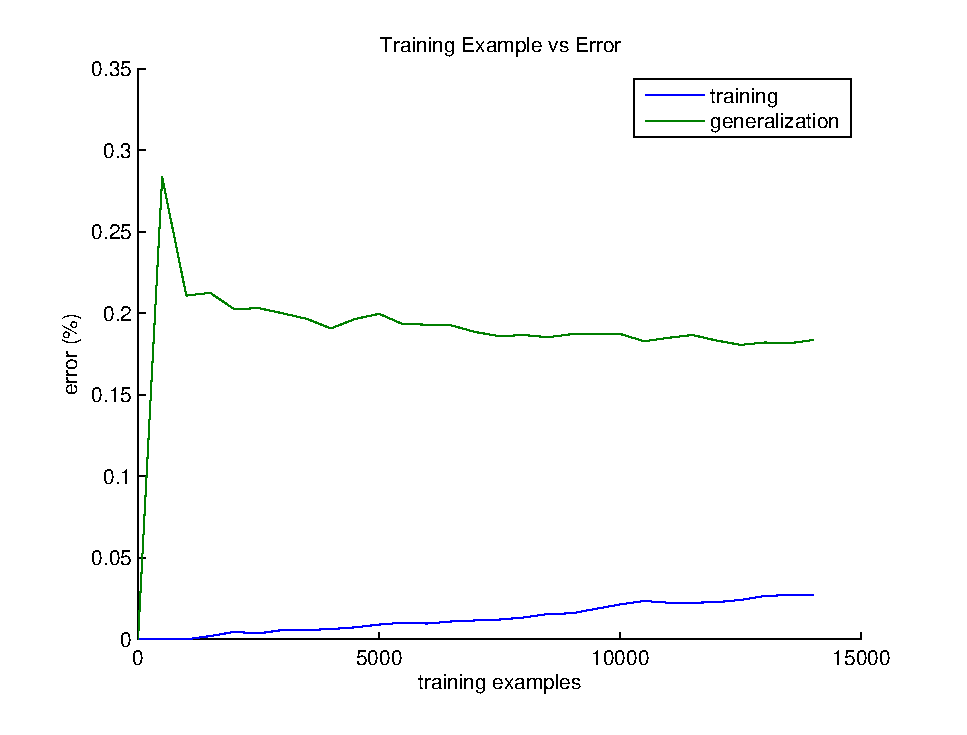
\includegraphics[scale=0.5]{logit-spell-bigram-error}
\par\end{center}


\subsection*{Discussion}

Individually, every data processing technique improved the generalization
accuracy but all of them with the exception of bi-grams, also reduced
training accuracy. When combined incrementally, however, it appears
that stemming and stopword removal actually reduces generalization
accuracy.

From the individual and incremental experiment results, we gathered
that the most promising data processing techniques are spell correction
and bi-grams. Thus we combined only those two and indeed we achieved
training and generalization accuracies that were superior to the rest.

Looking at the training error vs generalization error, it is as expected
that by adding more training examples, the training error (bias) goes
up where as the generalization error (variance) goes down. However
the trend suggests that as we add more training examples, training
error will continue to go up where as the generalization error will
likely flat off. Judging from this we will have to either explore
other pre-processing techniques, other learning algorithms, or other
tuning techniques.
